%----------------------------------------------------------------------------------------
%	PACKAGES AND OTHER DOCUMENT CONFIGURATIONS
%----------------------------------------------------------------------------------------

\documentclass{article}

\usepackage{fancyhdr} % Required for custom headers
\usepackage{lastpage} % Required to determine the last page for the footer
\usepackage{extramarks} % Required for headers and footers
\usepackage[usenames,dvipsnames]{color} % Required for custom colors
\usepackage{graphicx} % Required to insert images
\usepackage{listings} % Required for insertion of code
\usepackage{courier} % Required for the courier font
\usepackage{lipsum} % Used for inserting dummy 'Lorem ipsum' text into the template
\usepackage{url}
% Margins
\topmargin=-0.45in
\evensidemargin=0in
\oddsidemargin=0in
\textwidth=6.5in
\textheight=9.0in
\headsep=0.25in

\linespread{1.1} % Line spacing

% Set up the header and footer
\pagestyle{fancy}
\lhead{\hmwkAuthorName} % Top left header
\chead{\hmwkClass\ (\hmwkClassTime)} % Top center head
\rhead{\firstxmark} % Top right header
\lfoot{\lastxmark} % Bottom left footer
\cfoot{} % Bottom center footer
\rfoot{Page\ \thepage\ of\ \protect\pageref{LastPage}} % Bottom right footer
\renewcommand\headrulewidth{0.3pt} % Size of the header rule
\renewcommand\footrulewidth{0.4pt} % Size of the footer rule

\setlength\parindent{0pt} % Removes all indentation from paragraphs

%----------------------------------------------------------------------------------------
%	CODE INCLUSION CONFIGURATION
%----------------------------------------------------------------------------------------

\definecolor{MyDarkGreen}{rgb}{0.0,0.4,0.0} % This is the color used for comments
\lstloadlanguages{R} % Load Perl syntax for listings, for a list of other languages supported see: ftp://ftp.tex.ac.uk/tex-archive/macros/latex/contrib/listings/listings.pdf
\lstset{language=R, % Use Perl in this example
        frame=single, % Single frame around code
        basicstyle=\small\ttfamily, % Use small true type font
        breaklines=true,
        keywordstyle=[1]\color{Blue}\bf, % Perl functions bold and blue
        keywordstyle=[2]\color{Purple}, % Perl function arguments purple
        keywordstyle=[3]\color{Blue}\underbar, % Custom functions underlined and blue
        identifierstyle=, % Nothing special about identifiers                                         
        commentstyle=\usefont{T1}{pcr}{m}{sl}\color{MyDarkGreen}\small, % Comments small dark green courier font
        stringstyle=\color{Purple}, % Strings are purple
        showstringspaces=false, % Don't put marks in string spaces
        tabsize=5, % 5 spaces per tab
        %
        % Put standard Perl functions not included in the default language here
        morekeywords={},
        %
        % Put Perl function parameters here
        morekeywords=[2]{on, off, interp},
        %
        % Put user defined functions here
        morekeywords=[3]{test},
       	%
        morecomment=[l][\color{Blue}]{...}, % Line continuation (...) like blue comment
        numbers=left, % Line numbers on left
        firstnumber=1, % Line numbers start with line 1
        numberstyle=\tiny\color{Blue}, % Line numbers are blue and small
        stepnumber=5 % Line numbers go in steps of 5
}

% Creates a new command to include a perl script, the first parameter is the filename of the script (without .pl), the second parameter is the caption
\newcommand{\rscript}[2]{
\begin{itemize}
\item[]\lstinputlisting[caption=#2,label=#1]{#1.R}
\end{itemize}
}

%----------------------------------------------------------------------------------------
%	DOCUMENT STRUCTURE COMMANDS
%	Skip this unless you know what you're doing
%----------------------------------------------------------------------------------------

% Header and footer for when a page split occurs within a problem environment
\newcommand{\enterProblemHeader}[1]{
\nobreak\extramarks{#1}{#1 continued on next page\ldots}\nobreak
\nobreak\extramarks{#1 (continued)}{#1 continued on next page\ldots}\nobreak
}

% Header and footer for when a page split occurs between problem environments
\newcommand{\exitProblemHeader}[1]{
\nobreak\extramarks{#1 (continued)}{#1 continued on next page\ldots}\nobreak
\nobreak\extramarks{#1}{}\nobreak
}

\setcounter{secnumdepth}{0} % Removes default section numbers
\newcounter{homeworkProblemCounter} % Creates a counter to keep track of the number of problems

\newcommand{\homeworkProblemName}{}
\newenvironment{homeworkProblem}[1][Problem \arabic{homeworkProblemCounter}]{ % Makes a new environment called homeworkProblem which takes 1 argument (custom name) but the default is "Problem #"
\stepcounter{homeworkProblemCounter} % Increase counter for number of problems
\renewcommand{\homeworkProblemName}{#1} % Assign \homeworkProblemName the name of the problem
\section{\homeworkProblemName} % Make a section in the document with the custom problem count
\enterProblemHeader{\homeworkProblemName} % Header and footer within the environment
}{
\exitProblemHeader{\homeworkProblemName} % Header and footer after the environment
}

\newcommand{\problemAnswer}[1]{ % Defines the problem answer command with the content as the only argument
\noindent\framebox[\columnwidth][c]{\begin{minipage}{0.98\columnwidth}#1\end{minipage}} % Makes the box around the problem answer and puts the content inside
}

\newcommand{\homeworkSectionName}{}
\newenvironment{homeworkSection}[1]{ % New environment for sections within homework problems, takes 1 argument - the name of the section
\renewcommand{\homeworkSectionName}{#1} % Assign \homeworkSectionName to the name of the section from the environment argument
\subsection{\homeworkSectionName} % Make a subsection with the custom name of the subsection
\enterProblemHeader{\homeworkProblemName\ [\homeworkSectionName]} % Header and footer within the environment
}{
\enterProblemHeader{\homeworkProblemName} % Header and footer after the environment
}

\newcommand{\quotes}[1]{``#1''}
%----------------------------------------------------------------------------------------
%	NAME AND CLASS SECTION
%----------------------------------------------------------------------------------------

\newcommand{\hmwkTitle}{Midterm Exam I} % Assignment title
\newcommand{\hmwkDueDate}{10/02/2017, 10:00pm (ET)} % Due date
\newcommand{\hmwkClass}{Applied Data Mining} % Course/class
\newcommand{\hmwkClassTime}{Online} % Class/lecture time
\newcommand{\hmwkClassInstructor}{Instructor: Hasan Kurban} % Teacher/lecturer
\newcommand{\hmwkAuthorName}{Keith Hickman} % Your name

%----------------------------------------------------------------------------------------
%	TITLE PAGE
%----------------------------------------------------------------------------------------

\title{
\vspace{2in}
\textmd{\textbf{\hmwkClass:\ \hmwkTitle}}\\
\normalsize\vspace{0.1in}\small{Due\ on\ \hmwkDueDate}\\
\vspace{0.1in}\large{\textit{\hmwkClassInstructor\ }}
\vspace{3in}
}

\author{\textbf{\hmwkAuthorName}}
\date{\today} % Insert date here if you want it to appear below your name

%----------------------------------------------------------------------------------------

\begin{document}

\maketitle

%----------------------------------------------------------------------------------------
%	TABLE OF CONTENTS
%----------------------------------------------------------------------------------------

%\setcounter{tocdepth}{1} % Uncomment this line if you don't want subsections listed in the ToC

%\newpage
%\tableofcontents
\newpage

\section*{Directions}
This midterm exam is due Monday Oct 2, 2017 10:00p.m (ET). \textbf{OBSERVE THE  TIME}. Absolutely
no midterm exam will be accepted after that time. All the work must be your own.  I am providing the \LaTeX{} of this document too. You are not allowed to post questions related  to the midterm exam  on Canvas (Piazza/Discussion). The last question is a bonus question. If you think that  any of the questions is ambiguous, answer it as you understand and explicitly explain your approach.

%%%%%%%%%%%%%%%%%%%%%%%%%%%%%%%%%%

%PROBLEM  1
%%%%%%%%%%%%%%%%%%%%%%%%%%%%%%%%%%
\begin{homeworkProblem}[Problem 1 (20 pt.)]
 Load mydata.txt into R and answer the following questions:
\begin{enumerate}
\item How many entries are in the data set?
2000 observations of 5 variables $\ldots$

\item How many unknown or missing data are in the data set? 
There are 8 missing values

Remove the tuples with the missing values and call this data, clean.mydata. You will use clean.mydata to answer the questions below:

 \subsection{R script to find missing data}
\rscript{explore}{Sample R Script With Highlighting}

  \subsection{Count of missing values}
There are 8 missing values

\item Calculate mean and median of variable V2?
Mean/Median cannot be calculated, as V2 is a character in mydata

\item Find variance, standard deviation and interquartile range of variable V4? Answer here $\ldots$
Variance = 16.33867
Standard Deviation = 4.042112
IQR = 5.29
 
\item Create a bar plot that shows count of data points for  classes \quotes{1} and \quotes{2} (variable 5). Is the data skewed?
Yes, the data is significantly skewed below zero, and right-skewed. 

 \subsection{R script}
\rscript{explore}{Sample R Script With Highlighting}

 \subsection{Bar plot}
Place images here with suitable captions.
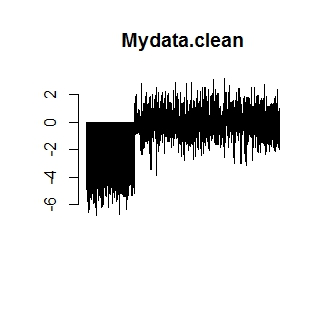
\includegraphics{problem1.jpeg}
 
  \subsection{Discussion of Data}
This data appears to be randomly generated. There are five variables, and it appears that V2 is the target class. $\ldots$

\item Create two scatter plots  using (1st, 2nd) and (1st, 3rd) variables and color the data points with the class variable (5th variable). Discuss the plots? Is there any pattern?


 \subsection{R script}
\rscript{scatter1}{Sample R Script With Highlighting}

 \subsection{Scatter plots}
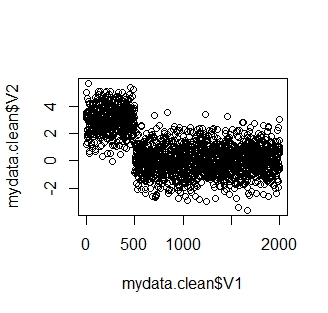
\includegraphics{scatter1_2.jpeg}
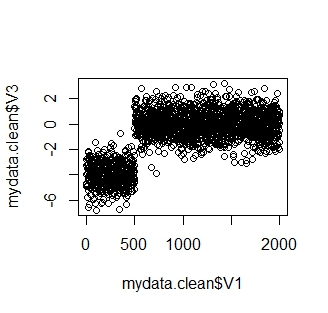
\includegraphics{scatter1_3.jpeg}
 
  \subsection{Discussion of Scatter Plots}


$\ldots$
\end{enumerate}
\end{homeworkProblem}




%%%%%%%%%%%%%%%%%%%%%%%%%%%%%%%%%

%PROBLEM 2
%%%%%%%%%%%%%%%%%%%%%%%%%%%%%%%%%%
\begin{homeworkProblem}[Problem 2 (20 pt.)]
Apply PCA to the clean.mydata and answer the following questions: (Remove the class variable, V5, before PCA)
\begin{enumerate}
\item How many principal components explain 90$\%$ of the variance? Answer here$\ldots$

 \subsection{R script}
\rscript{sb}{Sample R Script With Highlighting}
\item  What are loadings in PCA? Observe loadings and express the principal components using the original variables.

 \subsection{R script}
\rscript{sb}{Sample R Script With Highlighting}


 
  \subsection{Discussion and results}
Answer here$\ldots$

\item Make a scree plot. Discuss the plot, i.e., what is a scree plot? What is the optimal number of dimensions based on the plot? 

 \subsection{R script}
\rscript{sb}{Sample R Script With Highlighting}

 \subsection{Scree plot}
Place images here with suitable captions.
 =
  \subsection{Discussion}
Answer here$\ldots$

\item Make a scatter plot of PC2 and PC3. Do you observe any relationship? i.e., 
Calculate the correlation between PC2 and PC3? What does it show?
 \subsection{R script}
\rscript{sb}{Sample R Script With Highlighting}

 \subsection{Scatter plot}
Place images here with suitable captions.
 
  \subsection{Discussion}
Answer here$\ldots$

\end{enumerate}

\end{homeworkProblem}


%%%%%%%%%%%%%%%%%%%%%%%%%%%%%%%%%

%PROBLEM 3
%%%%%%%%%%%%%%%%%%%%%%%%%%%%%%%%%%
\begin{homeworkProblem} [Problem 3 (20 pt.)]

Run the R code below:


 \begin{verbatim}kmeans.mydata <- clean.mydata[,c(1,2)])\end{verbatim}

\begin{enumerate}
\item Randomly sample without replacement 300 data points from kmeans.mydata. (call the sampled data, mysample). Cluster mysample with $K$-means. Include the R  code and answer the questions below:

 \subsection{R script}
\rscript{sb}{Sample R Script With Highlighting}


\item  Explain $iter.max$  and $algorithm$ parameters of kmeans function in R and run $k$-means on mysample data set where $nstart = 35$  and $k=2$. Report total within squares error and  within squares error for each cluster.


 \subsection{R script}
\rscript{sb}{Sample R Script With Highlighting}


 
  \subsection{Discussion and results}
Answer here$\ldots$

\item Make a plot of data points and color the observation according to the cluster labels obtained. 

 \subsection{R script}
\rscript{sb}{Sample R Script With Highlighting}

 \subsection{Cluster plot}
Place images here with suitable captions.
 


\item  Run k-means on mysample data set where $nstart = 35$  and $k=4$. Report total within squares error and  within squares error for each cluster.

 \subsection{R script}
\rscript{sb}{Sample R Script With Highlighting}

 
  \subsection{Results}
Answer here$\ldots$
\item Make a plot of data points and color the observation according to the cluster labels obtained.

 \subsection{R script}
\rscript{sb}{Sample R Script With Highlighting}

 \subsection{Cluster plot}
Place images here with suitable captions.

\item Compare (2) and (4). Answer here$\ldots$

\end{enumerate}
 
\end{homeworkProblem}




%%%%%%%%%%%%%%%%%%%%%%%%%%%%%%%%%

%PROBLEM 4
%%%%%%%%%%%%%%%%%%%%%%%%%%%%%%%%%%
\begin{homeworkProblem} [Problem 4 (20 pt.)]
 The file \texttt{rainfalldataraw.txt} are data collected in a cloud-seeding experiment over the span of approximately seven years using five sites. Total rainfall is collected for a fixed, arbitrary, and uniform period of time where seeding is compared to unseeding.  In particular, 
\begin{itemize}
\item SEEDED is a Boolean $\{$U,S$\}$, U for unseeded and S for seeded.  
\item SEASON is a string indicating one of four seasons $\{$FALL, WINTER, SUMMER, SPRING$\}$
\item The remaining columns $\{$A,B,C,D,E$\}$ are the sites of experiments and the total rainfall recorded.  
\end{itemize}
\begin{enumerate}
\item In the listing below, which line number effectively reads the data into an \textsf{R} data.frame?
\begin{lstlisting}
teach <- read.table(file="c:/R/rainfalldataraw.txt", header=FALSE, sep=",")
teach <- read.table(file="c:/R/rainfalldataraw.txt", header=TRUE, sep=",")
teach <- read.table(file="c:/R/rainfalldataraw.txt", header=TRUE, sep="")
\end{lstlisting}
Answer here$\ldots$
\item Give a select operation on the data.frame that gives the rows whose E variable values are greater than 4, but less than 5.  
\subsection{R script}
\rscript{sb}{Sample R Script With Highlighting}
\item Give the  code that produces the histogram of variable D.
\subsection{R script}
\rscript{sb}{Sample R Script With Highlighting}
\item How many tuples (or records) are in the data? Answer here$\ldots$
\item Identify the data that is either missing or likely corrupted.
\subsection{R script to find missing data}
\rscript{sb}{Sample R Script With Highlighting}
 
  \subsection{Results for missing data}
Answer here$\ldots$

\item Preprocess the data, addressing the problems above and save the file as \texttt{rainfixed.txt} as a csv file.  Explain explicitly what you have done in preprocessing this file.

\subsection{R script for preprocessing data}
\rscript{sb}{Sample R Script With Highlighting}
 
  \subsection{Results  and discussion for preprocessing step}
Answer here$\ldots$
\item Using any techniques you've learned, answer this question to a policy maker:  \begin{quote} When there isn't enough rain, we lose a substantial amount of tax revenue, because farmers lose crops and livestock.  We think this cloud-seeding works and want to seed these areas A,B,C,D,E when the rainfall is significantly less than average.  What does your datamining tell us?\end{quote} State any explicit assumptions that you need to answer the question thoughtfully and fully.  You should provide ample evidence of a thorough analysis of the data. Answer here$\ldots$
\end{enumerate}

\end{homeworkProblem}


%%%%%%%%%%%%%%%%%%%%%%%%%%%%%%%%%

%PROBLEM 5
%%%%%%%%%%%%%%%%%%%%%%%%%%%%%%%%%%
\begin{homeworkProblem}[Problem 5 (10 pt.)]
Assume four pieces of data $x_1 = (.5,2000,-100); x_2 = (.2,3000,-200); x_3 = (4,4000,-100), x_4 = (.14,4400,-140)$.  You've been hired to datamine this data using Euclidean distance.  How would you preprocess this \textit{before} datamining and explain why.   What are the two closest data points? 
\begin{enumerate}
\item[]

 \subsection{R script}
\rscript{sb}{Sample R Script With Highlighting}

   \subsection{Discussion an Results}
Answer here$\ldots$

\end{enumerate}
\end{homeworkProblem}



%%%%%%%%%%%%%%%%%%%%%%%%%%%%%%%%%

%PROBLEM 6
%%%%%%%%%%%%%%%%%%%%%%%%%%%%%%%%%%

\begin{homeworkProblem} [Problem 6 (5 pt.)]
You're given a sample of data: 15,2,44,21,40,20,19,18.  Calculate the sample mean and sample variance. Answer here$\ldots$
%%%%%%%%%%%%%%%%%%%%%%%%%%%%%%%%%%
\begin{enumerate}
\item[]
 \subsection{R script}
\rscript{sb}{Sample R Script With Highlighting}
\end{enumerate}


\end{homeworkProblem}

%%%%%%%%%%%%%%%%%%%%%%%%%%%%%%%%%

%PROBLEM 7
%%%%%%%%%%%%%%%%%%%%%%%%%%%%%%%%%%

\begin{homeworkProblem} [Problem 7 (5 pt.)]

 Choose \textit{all} that apply. Which of the following statistical measures can  be observed on a box plot?
\begin{enumerate}
\item[(a)] Mode
\item[(b)] Mean
\item[(c)] Median
\item[(d)] Outliers
\item[(e)] Noise
\item[(f)]Maximum element
\item[(g)] Minimum element
\item[(h)] Variance or covariance.
\end{enumerate}

Answer here $\ldots$
\end{homeworkProblem}

%%%%%%%%%%%%%%%%%%%%%%%%%%%%%%%%%%
%PROBLEM 8
\begin{homeworkProblem}[Problem 8 (5 pt.)]

 Choose \textit{all} that apply.  The most common methods of removing outliers are:
\begin{enumerate}
\item[(a)]Removing tuples with missing values.
\item[(b)]Duplicating tuples without missing values.
\item[(c)] Observing the probability of existing values in \item[(d)] Assuming a uniform distribution on existing values, then populating values using this probability.
\item[(e)] Putting in \texttt{Null} and ignoring the value in the operations.
\end{enumerate}
\end{homeworkProblem}

Answer here $\ldots$

%%%%%%%%%%%%%%%%%%%%%%%%%%%%%%%%%%
%PROBLEM 9
\begin{homeworkProblem} [Problem 9(10 pt.)]

Swiss bank data contains various lengths measurements on 200 Swiss bank notes. Load the Swiss bank data as follows:


 \begin{verbatim}
> install.packages("alr3")
> library("alr3")
> head(banknote)
  Length  Left Right Bottom  Top Diagonal Y
1  214.8 131.0 131.1    9.0  9.7    141.0 0
2  214.6 129.7 129.7    8.1  9.5    141.7 0
3  214.8 129.7 129.7    8.7  9.6    142.2 0
4  214.8 129.7 129.6    7.5 10.4    142.0 0
5  215.0 129.6 129.7   10.4  7.7    141.8 0
6  215.7 130.8 130.5    9.0 10.1    141.4 0
 \end{verbatim}
 
 Use whatever graphical techniques you think appropriate to investigate whether there is any pattern or structure in the data. Do you observe something suspicious?
 
\begin{enumerate}
\item[]
 \subsection{R script}
\rscript{sb}{Sample R Script With Highlighting}


 \subsection{Plots}
Place images here with suitable captions.
 
  \subsection{Discussions}
Answer here$\ldots$
 \end{enumerate}
\end{homeworkProblem}





%%%%%%%%%%%%%%%%%%%%%%%%%%%%%%%%%%


%PROBLEM 10
\begin{homeworkProblem} [Bonus question (10 pt.)]

Here is some data taken from a website that measures where a person clicks on a page:

\begin{table}[h]
\centering
\begin{tabular}{ll}
\textsf{user} & \textsf{location} \\
1 & UL, UL, UL, LR, M\\
2 & UL, LR, M, M\\
3 & LL, UR, M, M
\end{tabular}
\end{table}
where UL = upper left, LR = lower right, M = middle, LL = lower left, LR = lower right.  Find the entropy of location.
\begin{enumerate}
\item[]

 \subsection{R script}
\rscript{sb}{Sample R Script With Highlighting}
 \end{enumerate}
\end{homeworkProblem}

\end{document}